%% This is an example first chapter.  You should put chapter/appendix that you
%% write into a separate file, and add a line \include{yourfilename} to
%% main.tex, where `yourfilename.tex' is the name of the chapter/appendix file.
%% You can process specific files by typing their names in at the 
%% \files=
%% prompt when you run the file main.tex through LaTeX.

\chapter{The Loop Gap Resonator}

As mentioned in the introduction, for many applied modalities within applications that use NV centers, the MW field (often denoted $B_1$ from NMR nomenclature), requires both high power and high uniformity to achieve high-fidelity quantum-state manipulation over the entire sample volume. As volumes are increased however, to maximize the number of NVs addressed without having a deleterious affect on the optimal measurement time, applying such a field becomes more difficult using standard approaches such as shorted coaxial loops \cite{clevenson2015broadband,chipaux2015magnetic}, microstrip waveguides \cite{andrich2017long,horowitz2012electron}, and 50 $\Omega$-terminated coaxial transmission lines \cite{li2010design,mrozek2015circularly,zhang2016microwave,zhang2018vector}. These broadband approaches allow arbitrary drive frequencies, however, the lack of resonant enhancement forces a compromise between the addressed volume and field strength. Section \ref{resonant_enhc} describes how planar lumped-element resonators such as split-ring resonators \cite{bayat2014efficient}, planar-ring resonators \cite{zhang2016microwave,sasaki2016broadband}, omega resonators \cite{twig2013ultra,horsley2018microwave,simpson2017electron}, and patch antennas \cite{zhang2016microwave} can improve coupling between the resonator and the NVs by resonantly enhancing the local $B_1$ field and thus enable MW driving over larger regions, but at the expense of bandwidth and thus, for an operational magnetometer, dynamic range. Additionally, planar resonators are shown to yield poor homogeneity in the planes normal to their surface and therefore lend themselves less to bulk magnetometry than to 2D imaging applications. To address this shortcoming 3D resonators and cavities can be employed such as enclosed metallic cavity resonators \cite{rose2017coherent}, enclosed dielectric resonators \cite{breeze2017continuous,floch2016towards,creedon2015strong}, open dielectric resonators \cite{kapitanova2017dielectric}, and three-dimensional lumped element resonators \cite{angerer2016collective}, which provide good field homogeneity and strong resonantly enhanced fields, but offer little to no optical access. Since all-optical initialization and readout is a primary benefit for many solid-state spin systems, including NV diamond \cite{doherty2013nitrogen}, such a trade-off is incompatible with many existing and envisioned applications \cite{schirhagl2014nitrogen}. 

To address this current shortcoming a three-dimensional tunable loop-gap resonator (LGR), based on the anode block of a cavity magnetron, is used to achieve desired MW drive strengths homogeneously over large areas. Additionally, its open geometry allows for good optical accessibility for interrogation volumes centered within the LGR cavity. Traditionally, the LGR has been used either as the anode block of cavity magnetrons \cite{collins1948microwave}, or as a low frequency (2-4 GHz) lumped element resonator for electron paramagnetic resonance (EPR) studies \cite{rinard2005loopgap}.  

\section{Resonant Enhancement of the MW field}\label{resonant_enhc}

The LGR acts classically like an underdamped oscillator. It stores MWs within the confines of its geometrical structure by allowing the energy to oscillate back and forth between an electric and magnetic potential. At resonance ($\omega_0$) the ratio of magnetic energy to electric energy is 1. The time $\tau_{ring}$ the energy can oscillate before its power is reduced by a factor of 1/e is characterized by a dimensionless quantity called the Q-factor. It's defined by the following ratio
\begin{equation}
Q = \omega_0 \frac{Stored Energy}{Power Loss}.
\end{equation}
If the resonator is therefore continuously fed by an external power source an enhancement of the stored energy occurs that is proportional to the Q-factor of the cavity. The magnitude of the magnetic flux within the center cavity (for a cylindrical resonator) is given by
\begin{equation} \label{B1approx}
|B_1| \approx  2\left[\frac{\upmu_0}{\omega V_r}\right]^{1/2} \cdot \sqrt{P_0} \cdot \sqrt{Q},
\end{equation}
where $\upmu_0$ is the vacuum permeability, $P_0$ is the power coupled to the resonator, $\omega$ is the angular frequency, and $V_r$ is the volume of the center loop. Therefore, high Q's can aid in achieving strong magnetic fields within the oscillator cavity at limited power input. Other considerations for maximizing field strength are the drive frequency and cavity volume.

%It's therefore clear that a resonant enhancement of the magnetic field amplitude is induced which is proportional to the square root of the Q-factor. 


\section{Model}

The following sections build a model of the LGR both as an equivalent circuit and as solutions to Maxwell's equations for the LGR's geometry. Figure \ref{LGR_geometry1} shows the LGR with geometrical parameters used in the following sections. The focus here lies on hole-and-slot type LGR resonators since this variation is designed and used in the rest of this thesis. Other types of resonators are shown in section \ref{LGRDesignSection} Figure \ref{LGR_variation}.


\begin{figure}[h!]
\centering
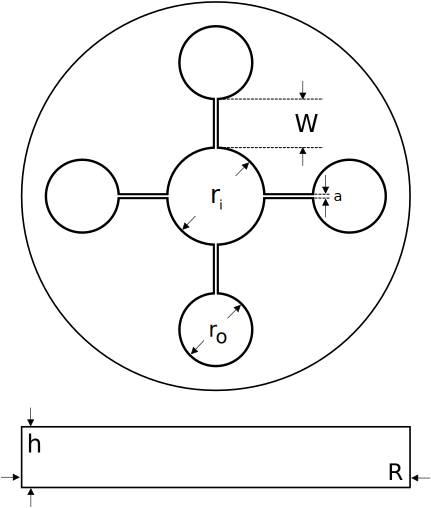
\includegraphics[scale = 0.7]{LGR_geometricalParams.pdf}  
\caption{\textbf{LGR dimensions} Geometrical parameters of LGR used in sections \ref{circuit} and \ref{fields}.}
\label{LGR_geometry1}
\end{figure}


\subsection{Equivalent circuit picture} \label{circuit}

\begin{figure}[t!]
\centering
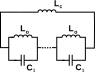
\includegraphics[scale = 1]{circuit_drawing.pdf}  
\caption{\textbf{LGR equivalent circuit diagram} Diagram showing equivalent inductance and capacitance of LGR and their connections.}
\label{circuitdiagram}
\end{figure}

The LGR can be modeled by an equivalent circuit in which the gaps behave like capacitors and the loops like inductors. It's important to note that such a picture neglects effects such as radiation losses or fringing fields that extend into space above and below the LGR. However, these effects can be incorporated with considerable effort and are described in detail within the following references \cite{mehdizadeh1983Loop, rinard2005loopgap, wood1984loop}. For an $m$ loop and $n$ gapped LGR, the equivalent circuit is depicted in Figure \ref{circuitdiagram}. Using the variables given in Figure \ref{LGR_geometry1}, the charge at the gap walls creates a capacitance $C_1$, and circulating currents around each loop create an inductance $L_1$
\begin{equation} \label{indcap}
C_1 \approx \frac{\epsilon_r \epsilon_0 W h}{a}, \quad L_1 \approx \frac{\mu_0 \pi r_i^2}{h}, 
\end{equation}
where $r_i$ is the radius of either loop ($i \equiv o,c$). Using circuit analysis and a simple approximation we can solve the diagram in Figure \ref{circuitdiagram} for the total capacitance, $C$,
\begin{equation}\label{capacitance}
C = \frac{C_1}{n},
\end{equation} 
and total inductance, $L$,
\begin{equation}\label{inductance}
L \approx \frac{n L_o L_i}{n L_o + L_i}.
\end{equation}
The resonant frequency of the LGR is then given by 
\begin{equation}
f_0 = \frac{1}{2 \pi \sqrt{LC}}
\end{equation}


\subsection{Solution to Maxwell's equations} \label{fields}

The full derivation of the solutions to Maxwell's equations for an $n$ gap LGR can be found in references \cite{piasecki1993field, mehdizadeh1989Electromagnetic, mehdizadeh1983investigation}. However, this section is intended to give a brief overview of the solutions, how they are attained, and how they can be used to estimate the field homogeneity and strength for an $n$ gap LGR. In general, Maxwell's equations for the LGR center cavity can be solved by using Bessel and Neumann functions which are found to be the solutions to finite length cylindrical waveguides \cite{gardiol1985open}. Neumann functions however are singular at the origin and therefore only Bessel functions (of the first kind) need to be considered. The magnetic field solution then takes the form
\begin{equation} \label{solution1}
B_z^{(p)} = \mathcal{J}_p(k\rho) e^{i p \phi}.
\end{equation}
Where we are operating in cylindrical coordinates and $\mathcal{J}_p$ is the $p^{th}$ order Bessel function and $k = \omega \sqrt{\mu_0\epsilon_0}$. If we assume that the field in the center loop is fully directed in $z$ then the magnetic field is simply
\begin{equation}\label{boundary1}
B_z = B_z(\rho,\phi)e^{i\omega t}, \quad B_{\rho} = B_{\phi} = 0.
\end{equation} 
The periodic boundary condition for the electric field is
\begin{equation}\label{maxwell1}
\begin{split}
E_\phi = 0 \quad \text{at} \quad \rho = r_c \\
& \text{for} \quad 2N\pi/n + \delta/2 \leqslant \phi \leqslant 2(N+1)\pi/n-\delta/2,
\end{split}
\end{equation}
and
\begin{equation}\label{maxwell2}
\begin{split}
E_\phi = E \quad \text{at} \quad \rho = r_c \\
& \text{for} \quad 2N\pi/n - \delta/2 \leqslant \phi \leqslant 2(N+1)\pi/n+\delta/2,
\end{split}
\end{equation}
where $N$ is an integer, $n$ is the number of gaps, and $\delta$ is the arc angle that is swept out by the capacitive gap, in radians. Additionally, we know from Maxwell's equations that
\begin{equation}\label{boundary2}
E_{\rho} = -i\frac{c \mu_0}{k \rho}\frac{\partial B_z}{\partial \phi},
\end{equation}
\begin{equation}\label{boundary3}
E_{\phi} =  i \frac{ c \mu_0}{k}\frac{\partial B_z}{\partial \rho}.
\end{equation}
Using equation \ref{solution1} in \ref{boundary2} and \ref{boundary3} and solving for the appropriate Bessel functions using the boundary conditions \ref{maxwell1} and \ref{maxwell2} yields, for the magnetic field only,
\begin{equation}
|B_z(\rho,\phi)| = - c \epsilon\mu_0 \frac{n E \delta}{2\pi} \times \left(\frac{\mathcal{J}_0(k\rho)}{\mathcal{J}_0(k r_c)} + 2 \sum\limits_{p = 1}^{\infty} \frac{\mathcal{J}_{np}(k \rho)}{\mathcal{J}_{n p} (k r_c)} \frac{sin(np\delta/2)}{np\delta/2}cos(np\phi)\right),
\end{equation}
where $E$ is the maximum field contained in the capacitive gap [Figure \ref{LGR_Electric}], and $\epsilon = \epsilon_r\epsilon_0$. In this case $\epsilon_r$ is given by the shim material used to tune the resonator (assuming it fully spans the width of the gap). To get an estimate of the field deviation between the maximum and minimum points we should examine the center and boundary cases (ie. $\rho = r_c$ and $\rho = 0$). At the cavity center we find,
\begin{equation} \label{fieldcenter}
|B_z(0,0)| \approx c \epsilon\mu_0 \frac{nE\delta}{\pi k r_c}
\end{equation}
and at the cavity sidewalls (choosing $\phi = 0$ for convenience),
\begin{equation}
|B_z(r_c,0)| \approx -c\epsilon\mu_0 \frac{nE \delta}{\pi} \left(-\frac{1}{k r_c}+ \frac{k r_c}{n}(1-\text{ln} n\delta/2)\right).
\end{equation}
To quantify the inhomogeneity we use the peak to peak variation $\sigma_{pp}$ defined as,
\begin{equation} \label{homogeneity}
\begin{split}
\sigma_{pp} = 2\frac{|B_z(0,0)| - |B_z(r_c,0)|}{|B_z(0,0)| + |B_z(r_c,0)|} \\
& \approx 2\frac{(kr_c)^2}{n}(1-\text{ln}n\delta/2)
\end{split}
\end{equation}
For the LGR used in this study (introduced and described in more detail in the sections to come) we can calculate $\sigma_{pp} \approx 8.9\%$ across the entire center loop when excited at 2.87 GHz. We will see in sections \ref{simField} and \ref{field} that this estimate is too low. This is likely due to the fact that the model described above neglects fringing field effects and thus assumes that the electric field has no axial variation and that the magnetic field is perfectly polarized in the z-direction. Furthermore, using equation \ref{fieldcenter} and the electric field information contained in figure \ref{LGR_Electric} we calculate the estimated field strength in the cavity center to be $B_z(0,0) \approx 2.2$ gauss which, referring to section \ref{simField} and \ref{LGRfield}, is too low an estimate. This most likely arises from the fact that the model above neglects any resonant enhancement of the field due to the cavity Q factor (see section \ref{resonant_enhc}).
%\subsection{Coupling} \label{coupling}

%Theory of coupling (mutual inductance, capcitance, etc)

\section{LGR Design} \label{LGRDesignSection}

Due to the loop gap resonator's usage in a variety of applications since the early 20th century \cite{collins1948microwave}, it has seen many variations and modifications. Figure \ref{LGR_variation} shows the cross section of a variety of LGRs including rising-sun, vane, slot, and hole-and-slot type resonators. EPR experiments at low frequencies (2-4 GHz) quickly adopted the LGR as opposed to more traditional TE\textsubscript{102} type cavities because of the LGR's smaller size relative to the wavelength of excitation. At 3 GHz the side length of the TE\textsubscript{102} cavity must be at least 5 cm which drastically reduces the cavity filling factor for small samples--a parameter necessary for the sensitivity of an EPR signal. Since many aspects of EPR spectroscopy are mirrored in NV magnetometry (requirement of homogeneous and strong microwave signals, frequency of operation, etc.) we selected to design a hole-and-slot type resonator. 
\vspace{5mm}
\begin{figure}[t!]
\centering
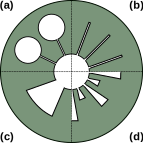
\includegraphics[scale = 0.5]{LGR_Variation.pdf}  
\caption{\textbf{Loop Gap Resonator Variations} \textbf{a)} Hole and Slot. \textbf{b)} Slot. \textbf{c)} Vane. \textbf{d)} Rising Sun - type}
\label{LGR_variation}
\end{figure}


\subsection{LGR}

A standard hole-and-slot LGR with $n$ outer loops can be approximated as $n$ coupled LC resonators oscillating in tandem at a target resonant frequency \cite{wood1984loop}. Circulating currents around the central and outer loops create a total inductance \ref{inductance}, and charge at the gaps creates the total capacitance \ref{capacitance} as found in section \ref{circuit}. In practice, the central loop diameter is set to $\sim 5-10 $ mm, corresponding to the typical size of a diamond plate. The outer loop diameters are chosen to match the inner diameters within a small factor to ensure return flux is captured and does not extend into the annular region around the LGR \cite{mehdizadeh1983Loop}. Since the outer and inner loops set the effective inductance of the resonator, the gap area $A = h \times W$ is constrained by the dual LGR design objectives of (i) maintaining optical accessibility, which limits the thickness of the device, and (ii) bounding $f_0$ above the target resonant frequency in order to allow for further tuning vie dielectric shims (discussed in section \ref{tuning}). Additionally, while increasing the number $n$ of loops and gaps can improve $B_1$ uniformity (see equation \ref{homogeneity}) and lower the LGR's resonant frequency, this approach results in a denser mode spectrum \cite{froncisz1982loop} and increases the likelihood of cross-mode excitations deleteriously altering the field distribution within the central loop. As a compromise, the design employs $n=4$ outer loops [Fig. \ref{LGR_drawing} (a)] allowing for sufficient uniformity while locating the closest eigenmode more than 2 GHz below the TE\textsubscript{10} eigenmode [Table \ref{eigenmodetable}].  

\begin{figure}[t!]
\centering
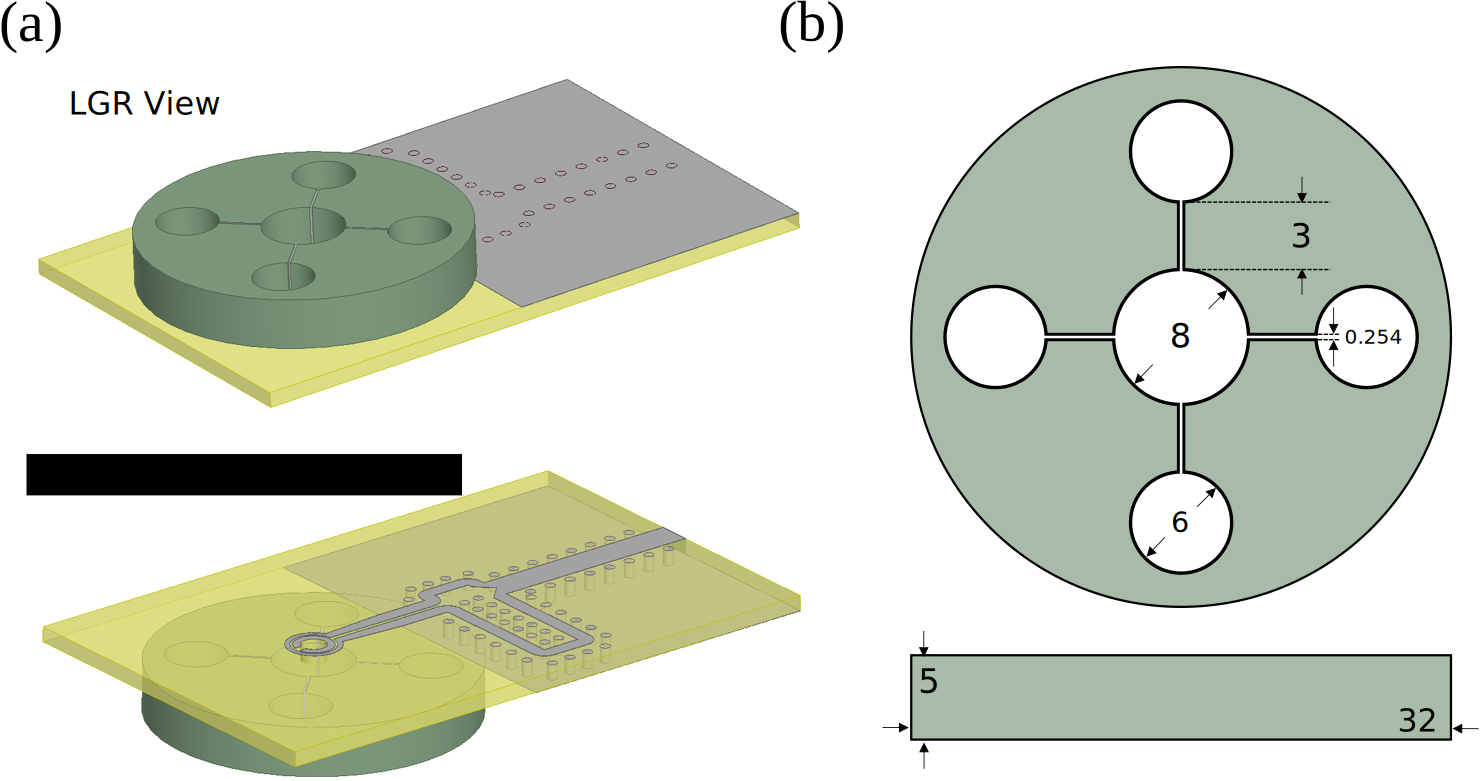
\includegraphics[width = \textwidth]{LGR_Image.pdf}  
\caption{\textbf{Rendering and Wire Diagram of Loop Gap Resonator} \textbf{a)} The metallic resonator employs a five-loop four-gap architecture. Microwaves are coupled into the LGR via the exciter antenna, which is fabricated on a printed circuit board. \textbf{b)} Line drawing of the LGR. All dimensions are in mm. Optional mounting holes and radial access port for laser excitation are now shown.}
\label{LGR_drawing}
\end{figure}

\begin{table}
\label{eigenmodetable}
\centering
   \begin{tabular}{llll} \hline Mode & freq. sim. \newline (GHz) & freq. meas. \newline (GHz) & figure \\
\hline 1 ($TE_{10}$) & \centering 4.6 & \centering 4.66 & \parbox[c]{1em}{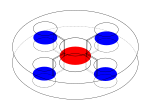
\includegraphics[width=1in]{Eigenmode1.pdf}} \\
2 & \centering 2.3 & \centering 2.53 & \parbox[c]{1em}{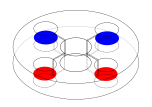
\includegraphics[width=1in]{Eigenmode2.pdf}} \\
3 & \centering 2.33 & \centering 2.51 & \parbox[c]{1em}{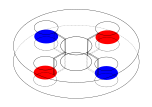
\includegraphics[width=1in]{Eigenmode4.pdf}} \\
4 & \centering $\sim 2$ & \centering 1 & \parbox[c]{1em}{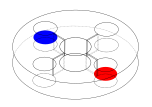
\includegraphics[width=1in]{Eigenmode3.pdf}} \\
\hline
\end{tabular}
\caption{Some modes the LGR supports and their measured vs. simulated frequencies. Many separate modes are degenerate due to their symmetrical nature. Additionally }
\end{table}

The LGR in this work therefore consists of a central loop with radius $r_c = 4$ mm surrounded by four symmetrically arranged outer loops of radius $r_o = 3$ mm as shown in Figure \ref{LGR_drawing} (b). The outer loops return magnetic flux to the central loop and therefore oscillate antisymmetrically with the central loop ($\pi$ out of phase). The side walls of the capacitive gaps are separated by $d = 254$ $\upmu$m. These dimensions, using equations \ref{indcap}, \ref{inductance}, and \ref{capacitance} yield $L = 8.7$ nH and $C = 0.17$ pF, resulting in an expected resonant frequency for the naked air-gapped LGR of $f_0 = 4.1$ GHz, approximately 1.2 GHz above the NV resonance frequencies. An eigenfrequency simulation of the resonator using the geometrical parameters listed above was completed in ANSYS HFSS and the distribution of the magnetic flux density ($B_1$) for the TE\textsubscript{10} mode is depicted in Figure \ref{LGR_Eigen}. As mentioned above, for this mode the center loop oscillates $\pi$ radians out of phase with the outer loops. The LGR however supports additional modes, some of which are depicted in Table \ref{eigenmodetable}. For the air-gapped resonator, HFSS returns a TE\textsubscript{10} real eigenfrequency at 4.57 GHz (depicted in Figure \ref{LGR_Eigen}). 

The LGR is fabricated via wire electron discharge machining, which is well-suited for producing the tight tolerances and vertical side walls required for the narrow $d = 254 \upmu$m capacitive gaps. A titanium alloy (Ti-6Al-4V) was chosen as the resonator cavity material. The lower conductivity of this alloy compared to that of copper ($\sigma_{Ti} = 5.8 \times 10^{5}$ S/m vs. $\sigma_c = 59 \times 10^6$ S/m) allows for a broader resonance with a 3dB bandwidth $\Delta_{3dB} = 80$ MHz, sufficient to address all eight NV resonances for bias magnetic fields $B_0$ up to $\sim 20$ gauss. This 80 MHz bandwidth corresponds to a loaded quality factor $Q_L \equiv f_0/\Delta_{3dB} \approx 36$ when the LGR
is critically coupled to the driving source (see section \ref{quality}). The LGR may be optionally fit with a radial access hole (for laser excitation of the NV ensemble) and three \# 2-56 mounting holes, which affix the LGR to an exciter antenna, discussed next.

\begin{figure}[h!]
\centering
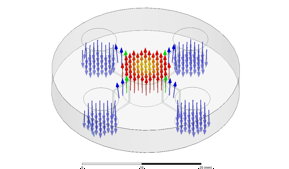
\includegraphics[scale = 0.6]{Eigen_Res.pdf}  
\caption{\textbf{Eigenfrequency solution to LGR} TE\textsubscript{10} mode located at $f_0 \approx 4.6$ GHz. The outer loops are oscillating $pi$ radians out of phase with center loop.}
\label{LGR_Eigen}
\end{figure}


\subsection{Tuning} \label{tuning}

The LGR resonant frequency $f_0$ is additionally tuned by inserting
and translating dielectric shims in the LGR's capacitive
gaps, thereby increasing the total capacitance C until $f_0$ overlaps the NV resonance frequencies as desired. Shimming material should be chosen to provide a high dielectric (and thus large tuning range) and low loss tangent (tan $\delta$, where $\delta$ is the inverse skin-depth). We employ 200 $\upmu$m thick C-plane sapphire, which is commercially
available in semiconductor grade 50.8 mm diameter wafers, can be cut on standard wafer dicing saws, has a high relative permittivity of $\epsilon_r = 11$ parallel to the C-plane \cite{westphal1972dielectric}, and exhibits a low dielectric loss of tan $\delta$ < 0.0001 at 3 GHz \cite{westphal1972dielectric, hartnett2006sapphireshim}. The sapphire shims are cut to lengths longer than the $l_c = 4$ mm radial length of the capacitive gaps, wedged into the gaps, and held in place with PTFE thread tape. These sapphire shims are then translated radially until the desired value of $f_0$ is attained. The shims are always positioned so that excess shim length extends into the outer rather than the central loop, in order to minimally perturb the central loop $B_1$ field. Simulations further suggest that radially symmetric shim configurations produce the best $B_1$ field homegoneity, as asymmetries in shim placement perturb the desired TE\textsubscript{01} field distribution. 



\subsection{Excitation Design} \label{excitation}

To couple MW power into the LGR two separate methods are utilized, each to be used for different NV applications. For magnetic  microscopy, complete 2$\pi$ steradian optical access to the center cavity is of the utmost importance. For such modalities lateral coupling using a shorted coaxial loop [Figure \ref{LGR_Lateral} (a)] can be used to minimize the blocking of optical access to the central loop \cite{koskinen1992the}. Using this method, resonator coupling is modified by changing the coaxial loop position in $z$ relative to the LGR. In this way the LGR can be quickly and effectively critically coupled for any shim configuration (ie. resonant frequency) [Figure \ref{LGR_Lateral} (b)]. Note that changing the coupling loop distance affects the mutual inductance between the shorted-loop and the resonator. As an undesired consequence, the resonant frequency of the total device shifts away from the frequency it was initially tuned to. A simple optimization process however, between shim placement and loop/LGR distance, can lead to the desired coupling at the targeted frequency.

\begin{figure}[t!]
\centering
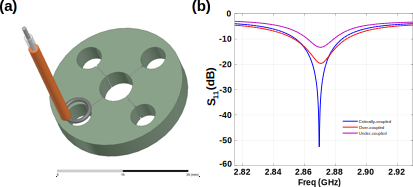
\includegraphics[width = \textwidth]{Lateral_Coupling.pdf}  
\caption{\textbf{3D Rendering of coupling loop and scattering parameter for different coupling configurations} \textbf{a)} Rendering of lateral coupling loop and LGR. \textbf{b)} Scattering parameter $S_{11}$ for different coupling configurations. Critically coupled (\textcolor{blue}{\textbf{---}}) at $z \approx 1$ mm, under-coupled (\textcolor{red}{---}) at $z \approx 1.25$ mm, over-coupled (\textcolor{purple}{---}). }
\label{LGR_Lateral}
\end{figure}

The purpose of the second devised coupling method is to provide a mechanically stable and wide bandwidth match for a future field-able NV magnetometer. While the lateral-loop coupling approach yields near perfect optical access to a sample placed in the center loop of the LGR, the long lever arm of the coaxial cable is susceptible to pertubation in a non-laboratory setting. An oscillation in the coupling loop manifests itself in an oscillation in the value of the coupling parameter $\beta$ and, in effect, an oscillation of the LGR resonant frequency and MWs supplied to the NVs. For applications that can sacrifice optical access, such as a bulk field-able magnetometer, A split-ring coupling structure is designed on a dielectric substrate which is subsequently mounted on the LGR [Figure \ref{LGR_drawing} (a)]. The fixed distance between the split-ring and LGR prevents quick "on-the-fly" coupling when the device is shim-tuned to another resonant frequency. Therefore the device must be well coupled across a wide bandwidth, which can be achieved using a balun (\textbf{ba}lanced-\textbf{un}balanced) placed between the feed-line and the exciter antenna (split-ring resonator). Figure \ref{LGR_Exciter} shows the exciter board composed of a 50:50 power splitter, a balun and a split-ring resonator. The balun is designed to match the exciter antenna to the LGR over a minimum bandwidth of 1 GHz centered at the zero-field splitting of the NV ($D_{gs}$). The 2D electromagnetic simulation tool Sonnet was used to ensure a flat $S_{21}$ and $S_{31}$ response between the feed-line and split-ring exciter antenna over the frequency range in question. 

\begin{figure}[t!]
\centering
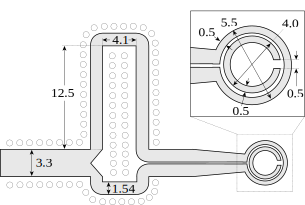
\includegraphics[scale = 0.45]{Exciter_Drawing.pdf}  
\caption{\textbf{Exciter board drawing} A feedline, 50:50 power splitter, and balun (\textbf{ba}lanced \textbf{un}balanced) feed the split ring resonator, which is coupled to the LGR. All dimensions are in mm. Optional mounting holes and radial access port for laser excitation are not shown}
\label{LGR_Exciter}
\end{figure}

Differential driving of the balun mitigates common-mode noise on the two traces, which might otherwise couple to the split-ring resonator. A via shield along a portion of the balun helps reduce interference and cross-talk between traces, controls trace impedance, and reduces radiative losses along the balun's $\pi$ phase delay arm. The exciter antenna is fabricated from a 1oz. copper trace with immersion silver finish on a 1.524 mm thick dielectric substrate (Rogers RO4350B). Although the proximity of the split-ring resonator perturbs the field distribution inside the LGR, both simulations and measurements suggest this effect is minimal and not the dominant source of inhomogeneity (See section \ref{field}).  

\begin{figure}[t!]
\centering
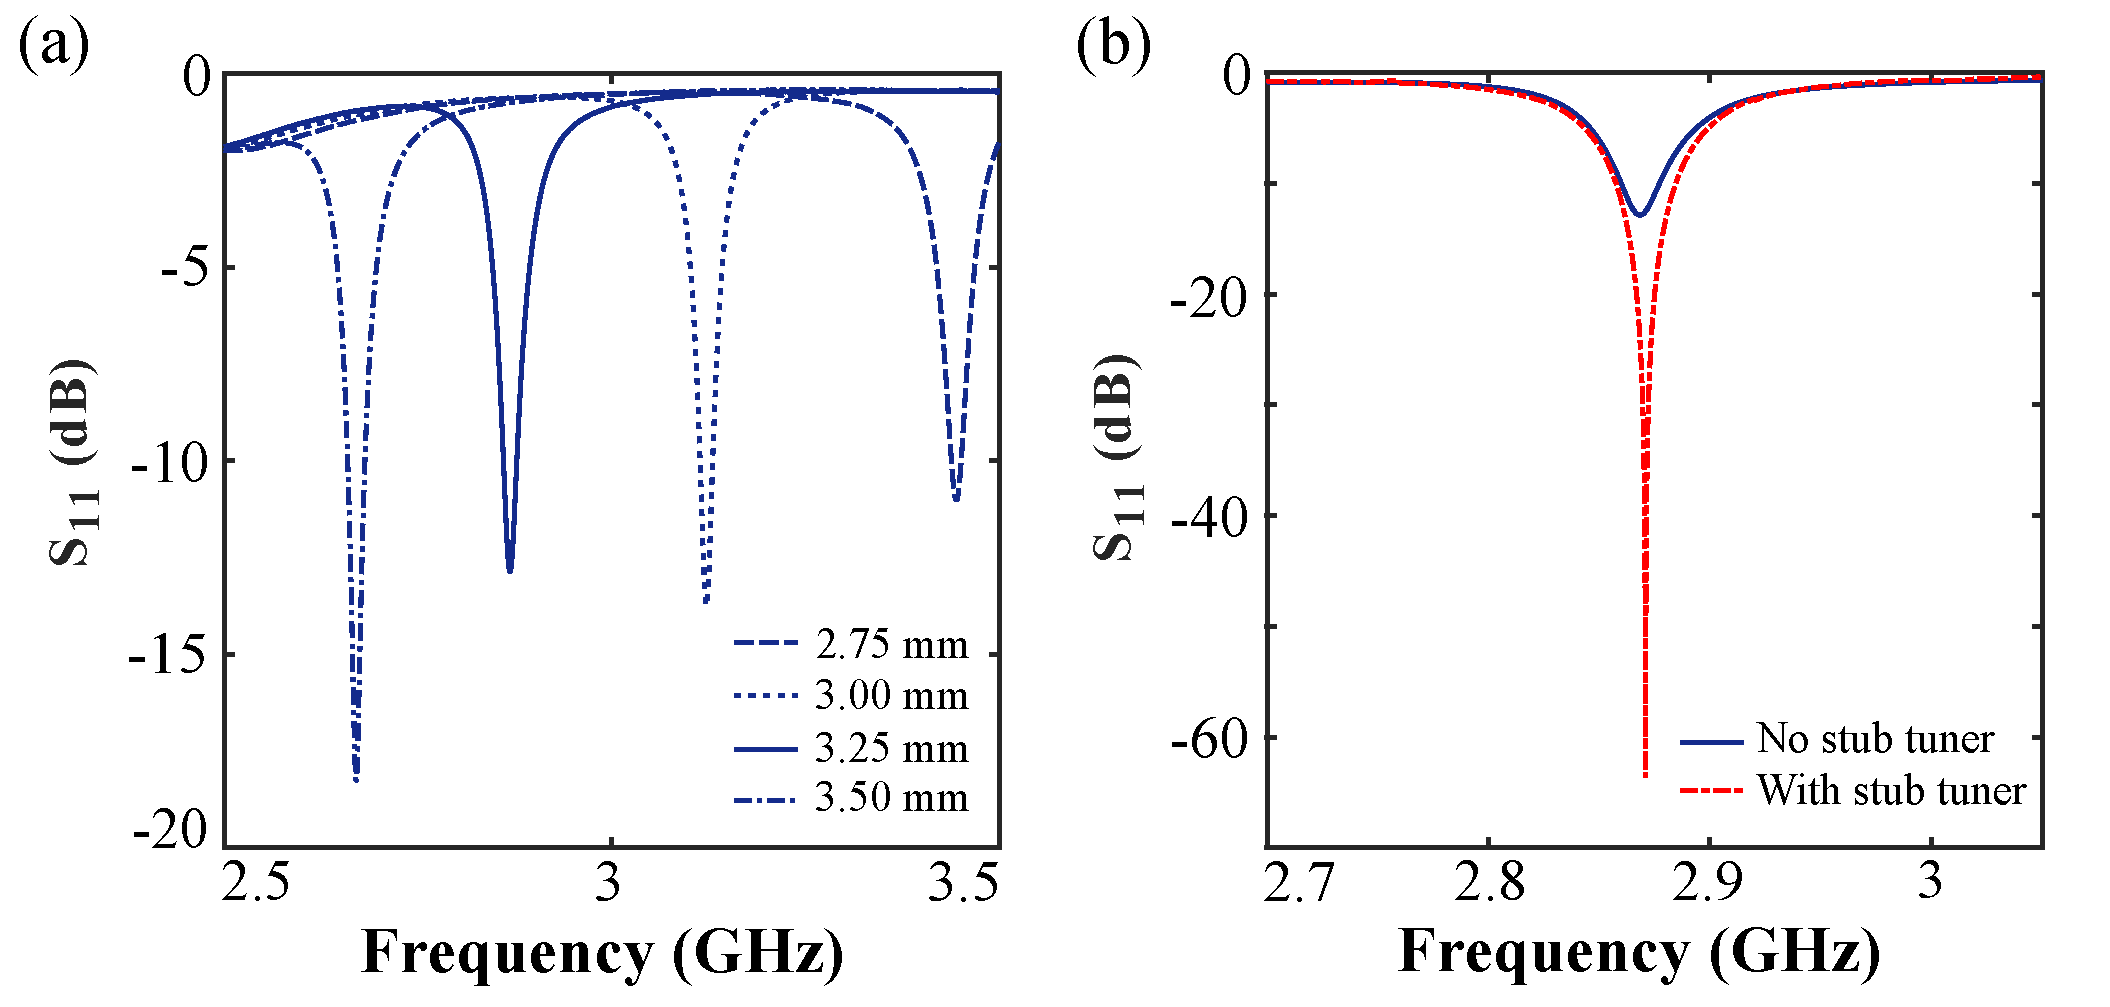
\includegraphics[width = \textwidth]{Figure_2.pdf}  
\caption{\textbf{Frequency tuning and impedance match-
ing of LGR composite device.} \textbf{(a)} The resonant frequency $f_0$ is adjusted by translating the sapphire shims in the four capacitive gaps. In the absence of a stub tuner, the LGR composite device exhibits $S_{11}$ values between -10 and -20 dB from 2.5 to 3.5 GHz, indicating at least $\gtrsim90\%$ of power delivered to the LGR composite device contributes to $B_1$ in this range. \textbf{(b)} Nearly perfect critical coupling can be achieved with
a stub tuner, allowing practically all incident MW power to contribute to $B_1$.}
\label{LGR_tuning}
\end{figure}

Although the microstrip balun is designed to match the feed-line and the split ring component of the exciter antenna at frequencies near 2.87 GHz, good matching is achieved from 2.5 GHz to 3.5 GHz as well. For drive frequencies between 2.5 and 3.5 GHz, the
exciter antenna board couples more than 90\% of incident MW power into the LGR, as shown in Figure \ref{LGR_tuning} (a). For a specific fixed frequency, the impedance matching may be further optimized by inserting a stub tuner between the MW source and the exciter antenna board, as shown in Figure \ref{LGR_tuning} (b). The stub tuner changes the effective electrical length of the exciter circuit and therefore modifies the coupling between the split ring resonator and the LGR. Similar matching can be achieved using a varactor diode instead of a stub tuner. 


%More robust coupling for implementable device

%Discussion of split ring exciter antenna and design outline of feedline and balun and design process of stepping through circuit etc.

%Talk about additional matching using stub tuner. 

%\begin{figure}[t!]
%\centering
%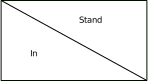
\includegraphics[width = \textwidth]{STANDIN.pdf}  
%\caption{\textbf{Eigenfrequency solution to LGR} \textbf{a)} \textcolor{red} {STANDIN. PLEASE REPLACE}}
%\label{LGR_Eigen}
%\end{figure}

\begin{figure}[t!]
\centering
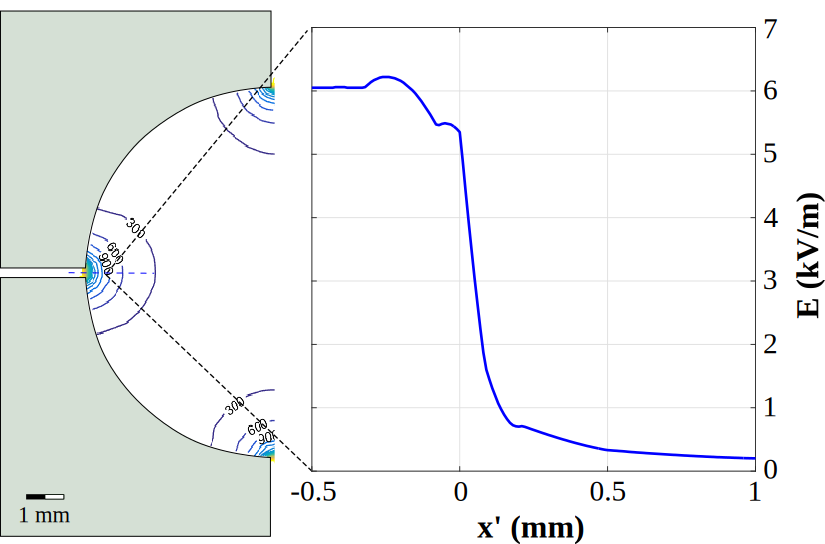
\includegraphics[scale = 0.55]{Figure_B_1.pdf}  
\caption{\textbf{Simulated electric field magnitude E in vicinity of LGR capacitive gap.} Inset depicts the electic field
magnitude E as a function of distance from the capacitive gap with $x' = 0$ mm corresponding to the plane of the central loop-gap interface.}
\label{LGR_Electric}
\end{figure}


\section{Electric Field}

One challenge that many MW solutions face is maintaining good coupling and a steady resonant frequency when a sample is introduced. For example, if a dielectric sample is placed on a planar resonator the dramatic change in capacitance between trace elements causes a shift in the resonant frequency \cite{bayat2014efficient, sasaki2016broadband, zhang2016microwave} of the oscillator. Just like planar fabricated resonators, the LGR is a lumped element device, but its large size permits an improved spatial separation between the electric and magnetic fields in the cavity. The electric field in the TE\textsubscript{10} mode is confined to the capacitive gaps and thus has little interaction with a dielectric sample placed in the center cavity. In practice, fringing electric Fields from the gaps extend partially into the LGR's central loop as shown in Figure \ref{LGR_Electric}. However, at distances > 1 mm from the capacitive gaps, the electric Field magnitude |E| is decreased by >10x from the peak Field inside the capacitive gap. Consequently, insertion of a diamond (with
$\epsilon_r \approx 5.7$ at 3 GHz \cite{ibarra1997wide}) beyond this region has little if any effect on the LGR resonant frequency $f_0$.

%\begin{figure}[h!]
%\centering
%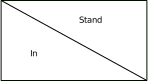
\includegraphics[width = \textwidth]{STANDIN.pdf}  
%\caption{\textbf{Electric field} \textbf{a)} \textcolor{red} {STANDIN. PLEASE REPLACE}}
%\label{LGR_Sample}
%\end{figure}

